\documentclass[12pt]{article}
\usepackage{xcolor}
\usepackage{fontspec}
\usepackage{booktabs}
\usepackage{csquotes}
\usepackage{langsci-gb4e}
\usepackage[style=langsci-unified,backend=biber]{biblatex}
\addbibresource{refs.bib}
\usepackage{amsmath}
\usepackage{amssymb}
\usepackage{tcolorbox}
\usepackage{tikz}
\usepackage{pgfplots}
\pgfplotsset{compat=1.18}
\usepackage{microtype}
\usepackage{float}
\usetikzlibrary{arrows.meta,shapes,positioning}
\usepackage{orcidlink}
\usepackage{hyperref}
\hypersetup{
    colorlinks=true,
    linkcolor=blue,
    filecolor=magenta,
    citecolor=blue,      
    urlcolor=cyan,
    pdftitle={Grammaticality as Kind},
    pdfpagemode=FullScreen,
}

\setmainfont{Charis SIL}

\definecolor{lsLightBlue}{RGB}{201,233,246}
\definecolor{lsDOIGray}{RGB}{0,0,0}


\title{Grammaticality as Kind: Ontology, Epistemology, and Empirical Pay-off}
\author{Brett Reynolds \orcidlink{0000-0003-0073-7195}\\Humber Polytechnic \& University of Toronto\thanks{I used ChatGPT o3 and Claude Opus 4 in drafting this version of the paper. I take responsibility for all content. \\This work is licensed under CC-BY 4.0}}
\date{\today}

\begin{document}
\maketitle

\begin{abstract}
\small
\noindent
Linguists appeal to \textit{grammaticality} as if it were a stable ontological target, but debates persist: is it a matter of rule compliance, usage frequency, competence, or merely an illusion? This paper argues that grammaticality is best understood as a homeostatic property-cluster (HPC) kind anchored in morphosyntactic form–meaning pairings and regimented by community practice. Drawing on contemporary metaphysics of science, I show how grammaticality exhibits the key features of HPC kinds: a cluster of co-occurring properties (acceptability judgements, processing patterns, community conventions), homeostatic mechanisms that maintain cluster stability (language acquisition, repair strategies, sociolinguistic policing), and systematic projectability supporting inductive generalization. This analysis clarifies why grammaticality supports explanatory and inductive generalization despite surface variation and gradience. The HPC framework predicts which phenomena will pattern with grammaticality (morphosyntactic violations, semantic mismatches at the syntax-semantics interface) versus those that won't (pure phonotactic violations, processing overload). By grounding grammaticality in both cognitive mechanisms and social practices, the account reconciles the apparent universality of particular constraints with the evident community-relativity of others. The framework has implications for methodology (validating judgment tasks while acknowledging their limits), theory (reconciling generative and usage-based evidence), and typology (predicting which \enquote{exotic} grammars can exist as stable linguistic systems).
\end{abstract}

\section{Introduction}

\subsection{The problem: What kind of thing is grammaticality?}

Consider three utterances that native English speakers consistently reject:

\ea
\ea[*]{\textit{I've finished it yesterday.}}
\ex[*]{\textit{How many years do you have?}\hfill[intended `how old are you']}
\ex[*]{\textit{Furiously sleep ideas green colorless.}}
\z
\z
Each violates something we call \enquote{grammaticality}, but the violations differ profoundly. The first shows a semantic mismatch between tense and time adverbial, the second seems semantically coherent but fails to match community expectations, and the third fails to evoke any coherent meaning. Meanwhile, speakers accept the semantically bizarre \textit{Colorless green ideas sleep furiously} and trained linguists classify the unprocessable \textit{The rat the cat the dog chased killed ate the cheese} as \enquote{grammatical}.

This variation poses a fundamental question: what kind of thing is grammaticality? The question isn't merely terminological. How we answer determines what counts as evidence, which methods are appropriate, and what explanations succeed. If grammaticality counts as a natural kind in Khalidi's causal-realist sense, perhaps instantiated as a homeostatic property-cluster (HPC) kind, then its explanatory machinery will differ radically from a purely social construction. Sorting out which label fits therefore shapes the evidence we look for and the explanations we accept.

\subsection{The proposal: Grammaticality as homeostatic property-cluster kind}

This paper argues that grammaticality is best understood as a homeostatic property-cluster (HPC) kind. Following \textcite{boyd1991realism}, HPC kinds are individuated not by necessary and sufficient conditions but by:

\begin{enumerate}
\item A cluster of properties that tend to co-occur
\item Homeostatic mechanisms that cause and maintain this clustering
\item Sufficient stability to support induction and explanation
\end{enumerate}

For grammaticality, the property cluster includes morphosyntactic well-formedness, semantic compatibility, processing viability, and community entrenchment. The homeostatic mechanisms include child language acquisition, adult repair strategies, and sociolinguistic policing. Together, these create sufficient stability for grammaticality to function as a scientific kind despite exhibiting gradience, variation, and change.

\subsection{The pay-off: Resolving persistent puzzles}

The HPC analysis resolves several persistent puzzles:

\textbf{Gradience within categories}: Like biological species, grammaticality exhibits internal variation while maintaining categorical distinctness. The framework predicts which types of gradience are compatible with kind-hood (processing difficulty, semantic anomaly) and which aren't (fundamental mapping failures).

\textbf{Community variation}: Different speech communities can have different grammaticality facts while participating in the same kind, just as different populations of a species can have different trait distributions while remaining conspecific.

\textbf{Diachronic stability}: The homeostatic mechanisms explain how grammaticality persists through language change, with some properties more essential than others.

\textbf{Methodological validity}: If grammaticality is an HPC kind, then convergent evidence from multiple methods (judgments, corpora, experiments) is exactly what we expect, validating the field's multi-method approach.

\section{Empirical Profile of Grammaticality}

Before determining which ontological category best fits grammaticality, we need to establish its empirical profile. What are the phenomena that any adequate account must explain?

\subsection{MMMG's five components}

The Morphosyntactic-Meaning Model of Grammaticality (MMMG) identifies five components that interact to determine grammaticality:

\begin{enumerate}
\item \textbf{Morphosyntactic pairings}: Conventional links between morphosyntactic forms and meanings
\item \textbf{Contextual compatibility}: Alignment between morphosyntactic meaning and contextual interpretation  
\item \textbf{Processing viability}: Ability to parse within memory and attention limits
\item \textbf{Community entrenchment}: Degree of conventionalization within the speech community
\item \textbf{Structural bans}: Categorical prohibitions on certain configurations
\end{enumerate}
These components generate two measures: objective grammaticality $G(u)\in[0,1]$ and subjective feeling of ungrammaticality $F(u)\in[-1,0]$. Mismatches between them explain grammatical illusions and processing effects.

\subsection{Diagnostic stability across tasks, speakers, and time}

If grammaticality forms a genuine kind, judgements should show stability across different measurement contexts. The empirical record confirms this:

\textbf{Cross-task convergence}: Acceptability ratings correlate with production frequencies, reading times, and neural responses. Sentences rated as ungrammatical show increased P600 ERP components and are avoided in production tasks \parencite{schutze2016}.

\textbf{Inter-speaker agreement}: Despite individual variation, speakers show remarkable convergence on core cases. Agreement is highest for structural violations (*\textit{Which did you buy car?}), moderate for semantic mismatches (*\textit{I've finished it yesterday}), and lowest for processing difficulties.

\textbf{Temporal persistence}: Longitudinal studies show grammaticality judgements remain stable within individuals over years. Historical corpora reveal that while specific constructions change frequency, the types of violations speakers avoid remain consistent.

This stability suggests grammaticality isn't merely epiphenomenal but reflects underlying regularities in how form--meaning pairings are constrained.

\subsection{Cross-dialectal convergence and bounded divergence}

Dialects provide natural experiments in how grammaticality varies. The patterns are revealing:

\textbf{Convergent constraints}: All English dialects reject determiner extraction (*\textit{Which did you buy car?}), reflexive matrix-subject antecedent in a subordinate clause (*\textit{John}\textsubscript{i} \textit{said that Mary praised himself}\textsubscript{i}), and singular determiners with plural head nouns (*\textit{I bought an oranges}).

\textbf{Systematic variation}: Dialectal differences follow predictable patterns. Negative concord (\textit{I didn't see nothing}) varies along social lines. Verb movement parameters create clustered differences between languages.

\textbf{Bounded possibility space}: Languages exhibit a can't-get-there-from-here landscape of grammatical variation. While most English dialects maintain relatively fixed word order, some allow greater flexibility in specific contexts. North-eastern English permits quotative inversion (\textit{said she}) and Belfast English allows focus-fronting patterns. Yet no variety permits completely free word order or arbitrary scrambling. This suggests that grammatical systems can only vary along certain evolutionary pathways; the homeostatic mechanisms that maintain existing patterns also constrain the directions of possible change. What we observe isn't a set of absolute universals but rather a topology of accessible and inaccessible regions in grammatical space.

The pattern~-- convergence on core structural principles with variation in specific implementations~-- matches what we'd expect from an HPC kind with both cognitive and social components.

\section{Kinds in Contemporary Metaphysics}

Understanding grammaticality's ontological status requires examining how contemporary metaphysics classifies kinds. Each framework offers tools for understanding grammaticality's nature.

\subsection{Natural kinds (causal-realist sense)}

Causal–realist accounts of natural kinds (e.g. \textcite{Khalidi2013}) hold that a category is natural when there are \emph{causal mechanisms} that (i) keep its members similar in scientifically salient ways and (ii) underwrite reliable inductions and explanations. Micro-structure can satisfy those conditions, but it is only \emph{one} possible source of causal cohesion; evolutionary, developmental, or social mechanisms may do the job just as well.

Gold and electrons remain paradigm cases: a stable micro-structure (atomic \#79, charge $-e$) causally explains their characteristic behaviours. But causal realism also counts biological species, whose members vary genetically, and even some social kinds when their stabilizing mechanisms are well enough understood. Importantly, \textcite{Khalidi2013} explicitly includes historical kinds, categories whose membership depends on causal-historical chains rather than intrinsic properties. Languages and linguistic features fit naturally into this expanded conception, as their identity depends on historical transmission and evolutionary modification rather than timeless essences.

On this view, grammaticality could qualify as natural provided that there are \emph{non-accidental causal links} tying together its diagnostic properties: acceptability profiles, repair patterns, ERP signatures, acquisition trajectories, and so on. The question is therefore not whether grammaticality has an immutable \enquote{essence}, but whether identifiable mechanisms~-- cognitive constraints, learning biases, community policing~-- continue to \emph{produce and stabilize} the same cluster of effects over time and across populations. Subsequent sections argue that the mechanisms in Fig.~\ref{fig:homeostasis} do just that, giving grammaticality the explanatory resilience Khalidi deems the hallmark of a natural kind.

\subsection{Social kinds: norm governance and collective intentionality}

Social kinds like \textit{money} or \textit{marriage} exist through collective recognition. As \textcite{Haslanger2012} argues, social kinds are constituted by social practices and the attitudes of participants. A piece of paper counts as money~-- acquires monetary status~-- because we collectively treat it as such.

Grammaticality shows clear social dimensions. Speech communities collectively recognize certain forms as acceptable. This recognition is maintained through socialization, education, and norm enforcement. The grammaticality of preposition choice varies by community: British English prefers \textit{at the weekend} while naïve speakers of American English require \textit{on the weekend}. What counts as grammatical depends partly on which speech community's norms one has internalized.

But grammaticality resists reduction to pure social construction. Speakers can't simply decide that \textit{*Sleep furiously ideas} is grammatical through collective agreement. Processing constraints and form--meaning mapping requirements impose limits on what communities can conventionalize. This suggests grammaticality involves both social and non-social components.

\subsection{Homeostatic property-cluster kinds as a subtype of natural kind}

Within the broader causal-realist framework, \textcite{boyd1991realism} introduced HPC kinds to handle cases like biological species that function as kinds despite lacking essential properties. Notably, HPC kinds are particularly well-suited for historical and evolutionary phenomena where identity depends on causal-historical processes rather than fixed essences. An HPC kind is characteried by:

\begin{enumerate}
\item \textbf{Property cluster}: A set of properties that tend to co-occur, though no single property is necessary or sufficient
\item \textbf{Homeostatic mechanisms}: Causal processes that create and maintain the clustering
\item \textbf{Accommodation}: The clustering accommodates inductive and explanatory practices
\end{enumerate}

Consider \textit{mammal} as an HPC kind. The property cluster includes viviparity, mammary glands, hair, warm-bloodedness, and specific bone structures. The homeostatic mechanisms include developmental programmes and evolutionary constraints. No single property is essential (monotremes lay eggs), but the cluster remains stable enough to support biological generalization.

This framework seems promising for grammaticality. The property cluster might include acceptability judgments, production patterns, processing profiles, and acquisition trajectories. The homeostatic mechanisms might include cognitive constraints, social transmission, and functional pressures. HPC allows for variation while maintaining kind integrity.

\textcite{Miller2021} extends this HPC framework to \emph{word-kinds}, demonstrating that words are stabilized by two interacting homeostatic mechanisms: speaker-internal lexical routines and community performance norms. As Miller explains, \enquote{the combined effects of these mechanisms explain the clustering of properties, and hence account for the observed homeostasis of the property clusters that partly define word-kinds} \parencite[p.~26]{Miller2021}. 

The present paper extends this causal-realist logic to the next structural tier: \emph{grammaticality itself} is the stable constellation of morphosyntactic pairings, compatibility relations, processing biases, and community entrenchment, kept in place by the mechanisms diagrammed in Fig.~\ref{fig:homeostasis} (acquisition, repair, policing). Thus word-level and sentence-level phenomena exemplify the \emph{same} metaphysical species of kind even though the properties and mechanisms appropriate to each level differ. Just as Miller's lexical routines maintain word stability, so too do acquisition and repair mechanisms maintain grammatical stability at the sentence level.

\subsection{Cognitive kinds: predictive processors modulated by an attentional hyperprior}

Cognitive–realist approaches individuate kinds by the algorithms they realize rather than by their physical substrate.  On the classic reading, \emph{grammaticality} would therefore be constituted by a dedicated parsing or constraint-satisfaction procedure.  That story, however, sits uneasily with evidence that complex linguistic structure can emerge from domain-general prediction machinery once learners attend selectively to communicative signals \parencite{ReynoldsEcho}.

I adopt a revised cognitive-kind view: the underlying realiser is the generic hierarchical predictor posited by predictive-processing theory, but its \emph{precision-weighting} is genetically biased toward ostensive, hierarchically rhythmic input.  This attentional hyperprior acts as a gain control on prediction errors, guaranteeing that linguistic patterns dominate learning while leaving the algorithms themselves wholly domain-general.%

Two consequences follow.

\begin{enumerate}
  \item \textbf{Universality with variation.}  The hyperprior is uniform across populations, explaining why every neurotypical child acquires some language.  Because the predictor is generic, cultural transmission can still shape the surface grammar, giving the observed cross-linguistic diversity.
  \item \textbf{Alignment with spandrel arguments.}  Human echolocation shows that general circuitry can support high-level competencies once attention is focused on the relevant cues.  Language, on this view, is the parallel case where evolution installed the attention filter in advance, rather than the algorithm itself \parencite[see esp.\ §\emph{Echolocation: Spandrels, Adaptations, and Evolutionary Insight}]{ReynoldsEcho}.
\end{enumerate}

Thus grammaticality still qualifies as a \emph{cognitive kind}, but its identity conditions lie in a precision-biased predictive processor, not in any language-specific parsing routine.  The account predicts (i) universal infant preferences for ostensive speech, (ii) failure of non-human vocal learners to exploit hierarchical rhythm in the same way, and (iii) successful in-silico acquisition when a comparable gain parameter is added, all of which are testable (cf. \textcite{ReynoldsEcho}, §§ 5--6).%


\section{Why Grammaticality Fits the HPC Template}

Having established grammaticality's empirical profile and surveyed ontological options, I now argue it constitutes an HPC kind. The argument proceeds by identifying the property cluster, homeostatic mechanisms, and projectability that characterize HPC kinds.

\subsection{Core causal properties}

The grammaticality cluster centres on three causal properties that tend to co-occur and mutually reinforce each other:

\subsubsection{Morphosyntactic pairings}

At the core lies the systematic pairing of morphosyntactic forms with meanings. These pairings aren't arbitrary but follow regular patterns:
\begin{itemize}
    \item Hierarchical structure maps to semantic composition
    \item Linear order maps to information structure  
    \item Morphological marking maps to grammatical features
\end{itemize}
When these pairings succeed, utterances feel grammatical. When they fail, as in \textit{*Furiously sleep ideas green colorless}, grammaticality collapses.

\subsubsection{Compatibility \texorpdfstring{$K(u)$}{K(u)}}

The compatibility function measures alignment between morphosyntactic meaning $\mu(u)$ and contextual meaning $\sigma(u)$. High compatibility occurs when:
\begin{itemize}
    \item Tense morphology aligns with temporal reference
    \item Argument structure matches verb semantics
    \item Agreement features show consistent values
\end{itemize}
The present perfect's incompatibility with past-time \textit{yesterday} (*\textit{I've seen it yesterday}) exemplifies low $K(u)$ despite successful pairing.

\subsubsection{Entrenchment \texorpdfstring{$C^{t}(u)$}{C\^{}t(u)}}

Community entrenchment captures the degree of conventionalization. Highly entrenched patterns:
\begin{itemize}
    \item Show rapid processing
    \item Resist change
    \item Transfer to new lexical items
\end{itemize}
The entrenchment difference explains why \textit{sneaked} and \textit{snuck} can coexist while *\textit{bringed} remains impossible.

\subsection{Cluster-homeostasis mechanisms}
Five mechanisms operating at distinct timescales maintain the grammaticality cluster:

\subsubsection{Bias-guided acquisition (ontogeny)}
    Domain-general prediction machinery, modulated by an attentional hyperprior for hierarchical rhythm \parencite{ReynoldsEcho}, extracts form--meaning pairings and rejects statistically unlicensed mappings. This gives rise to morphosyntactic pairings and baseline compatibility $K(u)$. Children's systematic avoidance of unattested patterns despite noisy input reveals how acquisition biases filter the hypothesis space.

\subsubsection{Interactive alignment (millisecond–turn)}
    In conversation, speakers converge automatically on syntactic frames and prune misalignments in real time \parencite{PickeringGarrod2004}. This stabilizes processing viability and flags violations for immediate repair. The mechanism explains why disfluencies cluster around grammatical violations and why speakers rapidly detect and correct structural errors in their own and others' speech.

\subsubsection{Exemplar consolidation (daily–lifetime)}
    High-precision tokens are preferentially replayed during sleep consolidation while low-precision ones decay \parencite{Mirkovic2016}. Over years this yields Zipfian frequency distributions that drive entrenchment $C^t(u)$. The mechanism predicts that frequently accessed constructions become increasingly automated while rare patterns remain effortful.

\subsubsection{Prestige-weighted selection (decade)}
    Variants associated with high-status speakers spread faster through communities \parencite{labov2001,eckert2000}, pushing some constructions toward categorical bans while allowing sociolinguistic stratification to persist at gradient margins. This explains why prescriptive norms can override frequency (stigmatizing common forms like double negatives) and why structural bans often correlate with social evaluation.

\subsubsection{Iterated cultural evolution (multi-generational)}
    The transmission bottleneck amplifies learnability biases and filters out mappings that exceed processing or memory constraints \parencite{Kirby2014}. This multi-generational ratchet explains why structural bans converge across dialects even as surface patterns diverge; only learnable patterns survive iterated transmission.

Figure~\ref{fig:homeostasis} schematizes how these five mechanisms continually stabilize the property cluster. Each operates at its characteristic timescale while contributing to the overall homeostasis that maintains grammaticality as a stable kind.


\begin{figure}[htbp]
\centering
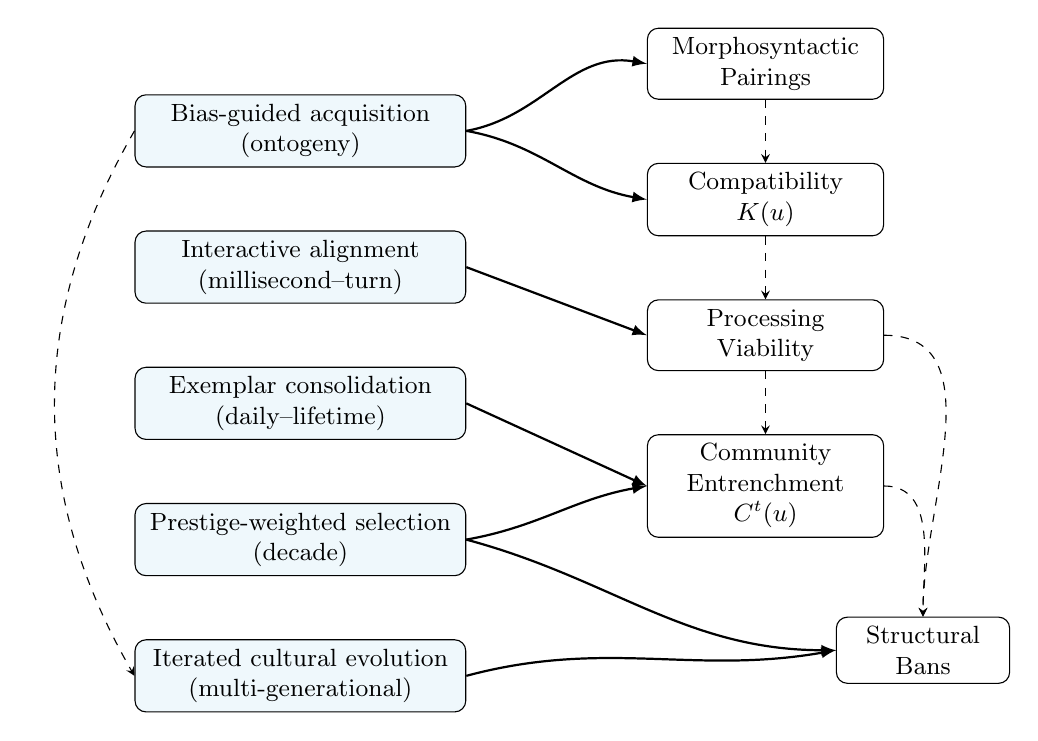
\begin{tikzpicture}[
  font=\small,
  node distance = 8mm and 22mm, % y-dist and x-dist
  mech/.style = {rectangle, draw, rounded corners,
                 minimum width=42mm, align=center, text depth=0.5ex,
                 fill=lsLightBlue!30},
  prop/.style = {rectangle, draw, rounded corners,
                 minimum width=30mm, align=center},
  bann/.style = {rectangle, draw, rounded corners,
                 minimum width=22mm, align=center},
  prim/.style = {->, >=latex, thick},
  sec/.style = {->, dashed, >={stealth}}
]

% Left Column: The 5 Mechanisms from the text
\node[mech] (acq)      {Bias-guided acquisition \\ (ontogeny)};
\node[mech, below=of acq] (align)    {Interactive alignment \\ (millisecond–turn)};
\node[mech, below=of align] (cons)     {Exemplar consolidation \\ (daily–lifetime)};
\node[mech, below=of cons] (prestige) {Prestige-weighted selection \\ (decade)};
\node[mech, below=of prestige] (iter)     {Iterated cultural evolution \\ (multi-generational)};

% An invisible coordinate is used to anchor the middle column for better alignment
\usetikzlibrary{calc}
\coordinate (mid_anchor) at ($(align)!0.5!(cons)$);

% Middle Column: Linguistic Properties
\node[prop, right=of mid_anchor, xshift=22mm] (proc) {Processing\\Viability};
\node[prop, above=of proc] (comp) {Compatibility\\$K(u)$};
\node[prop, above=of comp] (mp)   {Morphosyntactic\\Pairings};
\node[prop, below=of proc] (ent)  {Community\\Entrenchment\\$C^{t}(u)$};

% Right Column: Outcome
\node[bann, below=10mm of ent, xshift=20mm] (ban) {Structural\\Bans};

% Primary Causal Arrows (Solid) --- based on the paper's text
\draw[prim] (acq.east) to [out=10, in=170] (mp.west);
\draw[prim] (acq.east) to [out=-10, in=170] (comp.west);
\draw[prim] (align.east) to (proc.west);
\draw[prim] (cons.east) to (ent.west);
\draw[prim] (prestige.east) to [out=10, in=190] (ent.west);
\draw[prim] (prestige.east) to [out=-15, in=180] (ban.west);
\draw[prim] (iter.east) to [out=15, in=-170] (ban.west);

% Secondary Modulation Arrows (Dashed)
% Causal chain down the middle column
\draw[sec] (mp.south) to (comp.north);
\draw[sec] (comp.south) to (proc.north);
\draw[sec] (proc.south) to (ent.north);

% Properties influencing the final ban
\draw[sec] (ent.east) to[out=0, in=90] (ban.north);
\draw[sec] (proc.east) to[out=0, in=90] (ban.north); % Processing constraints filter mappings

% Feedback loop: learnability biases from acquisition are amplified by iterated evolution
\draw[sec, rounded corners] (acq.west) to [out=240, in=120] (iter.west);

\end{tikzpicture}
\caption{Homeostatic mechanisms stabilizing the grammaticality property-cluster. The five mechanisms (left) operate at different timescales to support a cluster of linguistic properties (middle), which collectively give rise to structural bans (right). Solid arrows denote primary causal support; dashed arrows show secondary modulation and feedback.}
\label{fig:homeostasis}
\end{figure}

\textbf{Projectability test.}  
Cross-linguistic ERP studies show that agreement violations elicit rapid
P600 or LAN effects not only in Germanic and Romance languages but also in Hindi
\parencite{Nevins2007}, Basque \parencite{Zawiszewski2009}, and Arabic
\parencite{MuralikrishnanIdrissi2021}. 
These convergent neural signatures confirm that the morphosyntactic–processing
link in Fig.~\ref{fig:homeostasis} travels with speakers across languages. 
Because acquisition, repair, and policing all funnel into maintaining reliable
agreement constraints, the same violation cues trigger comparable detection
responses, supporting the claim that grammaticality is a projectable
homeostatic kind.

\subsection{Projectability tests}

An HPC kind must support inductive and explanatory practices. Grammaticality passes three key tests:

\subsubsection{Predicting judgment patterns}

Knowing someone rejects \textit{*Which car did you buy car?} allows prediction they'll also reject:
\begin{itemize}
    \item \textit{*Which is charged phone?}
    \item \textit{*What will they make kind?}
    \item \textit{*This is the person whose you met brother.}
\end{itemize}
This projectability extends across construction types sharing abstract properties.

\subsubsection{S-curve diffusion}

The MMMG model predicts grammaticalizing constructions follow logistic growth curves. The entrenchment function $C^t(u)$ evolves according to:
$$\frac{dC^t}{dt} = r(u)C^t(1-C^t)$$
where $r(u)$ is the growth rate determined by factors including transparency, prestige, and analogical pressure. This generates S-shaped trajectories observed in historical changes like \textit{be going to} → \textit{gonna}. While detailed corpus verification awaits future work, the mathematical framework generates testable predictions about change rates.

\subsubsection{L2 error trajectories}

Second language learners show predictable acquisition sequences:
\begin{itemize}
    \item Initial reliance on L1 transfer
    \item Overgeneralization of L2 patterns  
    \item Gradual approximation to target norms
\end{itemize}
These trajectories support grammaticality's status as a learnable kind with systematic properties.

\section{Boundary Cases and Contrast Classes}

A complete account must explain not just what falls within the kind but what falls outside it. Two contrast cases illuminate grammaticality's boundaries:

\subsection{Processing overload: performance filter, not kind criterion}

Centre-embedded sentences like \textit{The rat the cat the dog chased killed ate the cheese} challenge the grammaticality/acceptability distinction \parencite[see esp. \S\S 2.2.7--2.2.8]{Gibson2024}:

\textbf{Intact form--meaning mapping}: Each embedded clause has a clear syntactic structure and semantic interpretation. The mapping succeeds in principle.

\textbf{Systematic processing failure}: The difficulty isn't random but predictable from memory constraints. Each embedding adds integration cost quantifiable as $\operatorname{ProcCost}(u) = \sum_{i} \operatorname{IntegrationDistance}(i)$ \parencite{gibson2000}.

\textbf{Amelioration strategies}: Unlike true ungrammaticality, processing difficulty can be reduced through prosody, context, or visual presentation.

\textbf{Competence/performance distinction maintained}: Speakers who can't process triple embedding still judge simpler versions grammatical, showing intact grammatical knowledge.

The processing/grammaticality distinction supports treating grammaticality as an HPC kind distinct from general cognitive constraints. When $F(u) \neq G(u)$, we observe mismatches between acceptability (performance-filtered) and grammaticality (the underlying competence system).

\subsection{Lexical anomaly: semantic oddity without kind violation}

\textit{Colorless green ideas sleep furiously} is semantically anomalous but grammatical. This boundary is principled:

\textbf{Successful form--meaning mapping}: Each morphosyntactic element contributes its expected meaning (plural morpheme \textit{-s} means `not one'; AdjP $\rightarrow$ Adj + AdvP means `property attribution under degree-modifier scope'). The oddity arises from combining these meanings, not from mapping failure.

\textbf{Metaphorical potential}: Unlike true ungrammaticality, semantic anomalies allow metaphorical rescue. \textit{Ideas sleep} could mean `ideas lie dormant'.

\textbf{No syntactic consequences}: Semantic anomaly doesn't block syntactic operations. We can form questions (\textit{Do colorless green ideas sleep furiously?}) and embed the clause (\textit{John thinks that colorless green ideas sleep furiously}).

\textbf{Cross-linguistic stability}: Languages agree on grammaticality but vary on semantic anomaly. What's metaphorically acceptable depends on cultural concepts.

\section{Objections}

Three major objections challenge the HPC analysis:

\subsection{The eliminativist challenge: grammaticality as fiction}

Eliminativists argue grammaticality is a pre-theoretical notion that scientific linguistics should abandon. On this view, speaking of \enquote{grammaticality} is like speaking of \enquote{phlogiston}, a theoretical posit that doesn't correspond to reality.

\textbf{Response}: The HPC framework doesn't require grammaticality to be a fundamental feature of reality. Like \textit{species} or \textit{gene}, grammaticality can be a non-fundamental kind that nonetheless plays an indispensable role in scientific explanation. The clustering of properties and the success of grammaticality-based generalizations justify maintaining the concept.

Moreover, eliminativism faces the challenge of explaining convergent judgements. If grammaticality were purely fictitious, why do speakers across cultures show such agreement? The HPC account explains this through shared cognitive mechanisms and functional pressures.

\subsection{The reductionist challenge: reduce to frequency or processing}

Reductionists claim grammaticality reduces to either usage frequency or processing ease. High-frequency patterns are grammatical; low-frequency or hard-to-process patterns are ungrammatical.

\textbf{Response}: While frequency and processing contribute to grammaticality, neither alone suffices:

\begin{itemize}
\item\textbf{Frequency}: Rare but grammatical constructions (\textit{This is Joan, }[\textit{a friend of whose}]\textit{ you met})\footnote{see \textcite{ReynoldsWhose}} show that low frequency doesn't entail ungrammaticality. Conversely, frequent errors in L2 speech almost never become grammatical through repetition.

\item\textbf{Processing}: Multiple centre-embeddings are unprocessable but grammatical. Simple violations like *\textit{I have two cat} process easily but remain ungrammatical. The dissociation shows these are distinct dimensions.
\end{itemize}
The HPC framework incorporates frequency (through entrenchment) and processing (through the $F(u)$ function) while maintaining grammaticality as an irreducible kind.

\subsection{The pluralist challenge: multiple kinds}

Pluralists argue that \enquote{grammaticality} names multiple distinct phenomena that shouldn't be unified. Perhaps morphological, syntactic, and semantic well-formedness are separate kinds.

\textbf{Response}: While grammaticality is internally complex, the phenomena show sufficient unity to constitute a single HPC kind:

\begin{itemize}
\item\textbf{Systematic interactions}: Morphological, syntactic, and semantic factors interact systematically. Agreement features are morphological but have syntactic distribution and semantic interpretation.

\item\textbf{Common acquisition path}: Children acquire these supposedly distinct systems in integrated fashion, suggesting underlying unity.

\item\textbf{Shared homeostatic mechanisms}: The same learning, processing, and social mechanisms maintain all aspects of grammaticality.
\end{itemize}
The HPC framework accommodates internal complexity while maintaining kind unity, just as \textit{mammal} includes monotremes and marsupials within a single kind.

\section{Implications}

Treating grammaticality as an HPC kind has implications for linguistic methodology, theory, and typology:

\subsection{Methodology: judgement tasks, corpora, ERP}

The HPC analysis validates methodological pluralism while explaining why different methods sometimes diverge:

\textbf{Acceptability judgements} tap the $F(u)$ function, which includes both grammatical and processing factors. High inter-speaker agreement on clear cases validates the method while variation on boundary cases is expected.

\textbf{Corpus frequencies} reflect production biases including processing cost, social indexicality, and discourse function alongside grammaticality. Absence from corpora doesn't entail ungrammaticality.

\textbf{Neural measures} like ERP show online processing correlates. P600 effects for violations validate grammaticality's psychological reality while showing it's not reducible to any single neural signature.

The framework predicts when methods will converge (clear violations of morphosyntactic pairing) and diverge (processing difficulties, socially stratified variants).

\subsection{Theoretical: reconciling generative and usage-based evidence}

The HPC framework suggests generative and usage-based approaches capture different aspects of the same kind:

\textbf{Generative insights}: The focus on structural constraints and categorical patterns captures the morphosyntactic core of the grammaticality cluster. Structural bans represent extreme points where homeostatic mechanisms maintain zero acceptability.

\textbf{Usage-based insights}: The focus on frequency, exemplars, and gradience captures entrenchment dynamics and social variation. S-curve diffusion shows how usage patterns feed back into grammatical knowledge.

Rather than choosing sides, the field benefits from recognising these as complementary perspectives on a complex kind.

\subsection{Typology: predicting which \enquote{exotic} grammars can exist}

The HPC analysis makes testable predictions about possible human languages:

\textbf{Permitted variation}: Languages can vary in:
\begin{itemize}
    \item Which semantic distinctions receive morphosyntactic marking
    \item How social factors influence entrenchment  
    \item Where processing limitations create acceptability gradients
\end{itemize}

\textbf{Prohibited variation}: Languages cannot:
\begin{itemize}
    \item Lack systematic form--meaning pairings entirely
    \item Have grammars unlearnable through the standard acquisition mechanism
    \item Violate processing constraints beyond recoverable limits
\end{itemize}
These predictions follow from grammaticality's homeostatic mechanisms. Any pattern incompatible with child acquisition, adult processing, or social transmission cannot stabilize as a grammatical system.

\section{Conclusion}

This paper has argued that grammaticality is a natural kind, realized as a homeostatic property-cluster (HPC) kind. Like biological species, grammaticality exhibits clustered properties maintained by identifiable mechanisms without reducing to essential features. The analysis resolves longstanding puzzles about gradience, variation, and the competence/performance distinction while validating linguistics' methodological practices.

The HPC framework reveals grammaticality as neither purely natural nor purely social but as emerging from the interaction of cognitive constraints, social conventions, and functional pressures. This perspective suggests that debates between formalist and functionalist approaches may rest on false dichotomies~-- grammaticality is the kind of complex phenomenon that requires both types of explanation.

Future work should explore how the homeostatic mechanisms operate across different linguistic levels, how the property cluster varies cross-linguistically, and whether other linguistic kinds (phoneme, word, construction) yield to similar analysis. The framework also opens questions about how grammaticality kinds relate to kinds in adjacent sciences~-- are there deep homologies between linguistic and biological evolution?

By taking grammaticality's ontology seriously, we gain insight into why human languages exhibit the particular mix of universality and diversity they do. The homeostatic mechanisms that maintain grammaticality also constrain its variation, explaining why all languages are both strange and familiar~-- different instantiations of the same fundamental kind.

\newpage
\begin{sloppypar}
\printbibliography[title=References]
\end{sloppypar}

\end{document}